%%%%%%%%%%%%%%%%%%%%%%%%%%%%%%%%%%%%%%%%%
% Beamer Presentation
% LaTeX Template
% Version 1.0 (10/11/12)
%
% This template has been downloaded from:
% http://www.LaTeXTemplates.com
%
% License:
% CC BY-NC-SA 3.0 (http://creativecommons.org/licenses/by-nc-sa/3.0/)
%
%%%%%%%%%%%%%%%%%%%%%%%%%%%%%%%%%%%%%%%%%

%----------------------------------------------------------------------------------------
%	PACKAGES AND THEMES
%----------------------------------------------------------------------------------------

\documentclass{beamer}

\newcommand{\EMSE}{ {\rm EMSE}}
\newcommand{\CC}{ {\rm CC}}
\newcommand{\MSE}{ {\rm MSE}}
\newcommand{\WIN}{\scriptscriptstyle {\rm WIE}}
\newcommand{\OROI}{\scriptscriptstyle {\rm out ROI}}
\newcommand{\Her}{\scriptscriptstyle H}
\newcommand{\T}{\scriptscriptstyle T}
\newcommand{\LMS}{\scriptscriptstyle {\rm LMS}}
\newcommand{\RDE}{\scriptscriptstyle {\rm RDE}}
\newcommand{\MRD}{\scriptscriptstyle {\rm MRD}}
\newcommand{\MSD}{\scriptscriptstyle {\rm MSD}}
\newcommand{\SBD}{\scriptscriptstyle {\rm SBD}}
\newcommand{\SDD}{\scriptscriptstyle {\rm SDD}}
\newcommand{\WIE}{\scriptscriptstyle {\rm WIE}}
\newcommand{\R}{\scriptscriptstyle {\rm R}}
\newcommand{\I}{\scriptscriptstyle {\rm I}}
\newcommand{\mT}{\scriptscriptstyle -T}
\newcommand{\vir}{,\hspace{-0.15ex}}
\newcommand{\M}{\scriptscriptstyle M}
\newcommand{\MMA}{\rm \scriptscriptstyle MMA}
\newcommand{\neigh}{\scriptscriptstyle {\rm neigh}}
\newcommand{\st}{\scriptscriptstyle {\rm st}}
\newcommand{\nd}{\scriptscriptstyle {\rm nd}}
\newcommand{\CSD}{\scriptscriptstyle {\rm CSD}}
\newcommand{\E}{{\rm E}}
\newcommand{\uM}{{\mathbf u}}
\newcommand{\rM}{{\mathbf r}}
\newcommand{\xM}{{\mathbf x}}
\newcommand{\yM}{{\mathbf y}}
\newcommand{\XM}{{\mathbf X}}
\newcommand{\w}{{\mathbf w}}
\newcommand{\wo}{{\mathbf{w}}_{\rm o}}
\newcommand{\q}{{\mathbf q}}
\newcommand{\qp}{{\mathbf {\dot{q}}}}
\newcommand{\Nuquad}{\|{\mathbf u(n)}\|^2}
\newcommand{\NuquadP}{\|{\mathbf u(n)}\|^2_{{\mathbf R}^{-1}(n)}}
\newcommand{\uMc}{{\mathbf u}^{\ast}}
\newcommand{\wtil}{\widetilde{\mathbf w}}
\newcommand{\Dw}{\boldsymbol{\Delta}{\mathbf w}}
\newcommand{\Dewp}{\boldsymbol{\Delta}{\mathbf{\dot{w}}}}
\newcommand{\Pb}{{\mathbf R}^{-1}}
\newcommand{\ebari}{{\bar{e}}_i}
\newcommand{\field}[1]{\mathbb{#1}}
\newcommand{\re}{\field{R}}
\newcommand{\co}{\field{C}}
\newcommand{\CO}{\field{C}}
\newcommand{\RE}{\field{R}}
\newcommand{\Tr}{{\rm Tr}}
\newcommand{\Ru}{{\mathbf R}}
\newcommand{\sgbeta}{\sigma_{\scriptscriptstyle{\!\alpha}}^2}
\newcommand{\sgphi}{\sigma_{\scriptscriptstyle{\!\varphi}}^2}
\newcommand{\cred}{\textcolor{red}}
\newcommand{\lbo}{\lambda_{\rm o}}
\newcommand{\cond}{\mathbf{w}_1(n\!-\!1),\mathbf{w}_{2}(n\!-\!1)}
\newcommand{\cb}{\textcolor{blue}}
\newcommand{\pu}{\mathbf{p}_{\!\scriptscriptstyle \Delta}}
\definecolor{laranja}{rgb}{0.8,0.5,0}
\newcommand{\crt}{\textcolor{laranja}}
\newcommand{\Psibf}{\boldsymbol{\Psi}}
\newcommand{\Sigmabf}{\boldsymbol{\Sigma}}
\newcommand{\epsbf}{\boldsymbol{\epsilon}}
\newcommand{\betabf}{\boldsymbol{\beta}}
\newcommand{\alphabf}{\boldsymbol{\alpha}}
\newcommand{\thetabf}{\boldsymbol{\theta}}
\newcommand{\gammabf}{\boldsymbol{\gamma}}
\newcommand{\lambdabf}{\boldsymbol{\lambda}}
\newcommand{\ML}{{\rm ML}}
\newcommand{\LS}{{\rm LS}}
\newcommand{\SSS}{{\rm SS}}
\newcommand{\UPS}{{\rm UPS}}
\newcommand{\PS}{{\rm PS}}

\mode<presentation> {

% The Beamer class comes with a number of default slide themes
% which change the colors and layouts of slides. Below this is a list
% of all the themes, uncomment each in turn to see what they look like.

%\usetheme{default}
%\usetheme{AnnArbor}
%\usetheme{Antibes}
%\usetheme{Bergen}
%\usetheme{Berkeley}
%\usetheme{Berlin}
%\usetheme{Boadilla}
\usetheme{CambridgeUS}
%\usetheme{Copenhagen}
%\usetheme{Darmstadt}
%\usetheme{Dresden}
%\usetheme{Frankfurt}
%\usetheme{Goettingen}
%\usetheme{Hannover}
%\usetheme{Ilmenau}
%\usetheme{JuanLesPins}
%\usetheme{Luebeck}
%\usetheme{Madrid}
%\usetheme{Malmoe}
%\usetheme{Marburg}
%\usetheme{Montpellier}
%\usetheme{PaloAlto}
%\usetheme{Pittsburgh}
%\usetheme{Rochester}
%\usetheme{Singapore}
%\usetheme{Szeged}
%\usetheme{Warsaw}

% As well as themes, the Beamer class has a number of color themes
% for any slide theme. Uncomment each of these in turn to see how it
% changes the colors of your current slide theme.

%\usecolortheme{albatross}
%\usecolortheme{beaver}
%\usecolortheme{beetle}
%\usecolortheme{crane}
%\usecolortheme{dolphin}
%\usecolortheme{dove}
%\usecolortheme{fly}
%\usecolortheme{lily}
%\usecolortheme{orchid}
%\usecolortheme{rose}
%\usecolortheme{seagull}
%\usecolortheme{seahorse}
%\usecolortheme{whale}
%\usecolortheme{wolverine}

%\setbeamertemplate{footline} % To remove the footer line in all slides uncomment this line
\setbeamertemplate{footline}[page number] % To replace the footer line in all slides with a simple slide count uncomment this line

\setbeamertemplate{navigation symbols}{} % To remove the navigation symbols from the bottom of all slides uncomment this line
}

\usepackage{graphicx} % Allows including images
\usepackage{booktabs} % Allows the use of \toprule, \midrule and \bottomrule in tables
\usepackage{color}
\usepackage{amsmath}
%----------------------------------------------------------------------------------------
%	TITLE PAGE
%----------------------------------------------------------------------------------------

\title[TopicModel]{Exploring and understanding documental databases with topic models and graph analysis} % The short title appears at the bottom of every slide, the full title is only on the title page

\author{Jer\'onimo Arenas-Garc\'{\i}a, Vanessa G\'omez-Verdejo, Jes\'us Cid-Sueiro} % Your name
\institute[UC3M] % Your institution as it will appear on the bottom of every slide, may be shorthand to save space
{
Universidad Carlos III de Madrid \\ % Your institution for the title page
\medskip
\textit{jeronimo.arenas@uc3m.es} % Your email address
}
\date{August 31, 2017}
%\date{\today} % Date, can be changed to a custom date

\begin{document}

%######################################################
%######################################################
\begin{frame}
\titlepage % Print the title page as the first slide
\end{frame}


%######################################################
%######################################################
\begin{frame}

    \frametitle{Contents}

	\large

    \begin{enumerate}
  
    	\item {\bf \color{blue}{Overview and block objectives}}
    	\item Corpus acquisition
    	\item Corpus preprocessing, cleaning and homogeneization
    	\item Topic modeling with Latent Dirichlet Allocation
    	\item Graph tools
    
    \end{enumerate}

\end{frame}

%######################################################
%######################################################
\section{1. Overview and block objectives}
\subsection{NLP}

%######################################################
%######################################################
\begin{frame}

	\frametitle{Natural Language Processing (NLP)}
	
	\begin{block}{Definition}
	\begin{itemize}
		\item Computer aided text analysis of human language
		\item The goal is to enable machines to understand human language and extract meaning from text
	\end{itemize}
	\end{block}
	
	This is a field of study which falls under the intersecting interests of (at least):
	\begin{itemize}
		\item machine learning
		\item computational linguistics
	\end{itemize}

\centerline{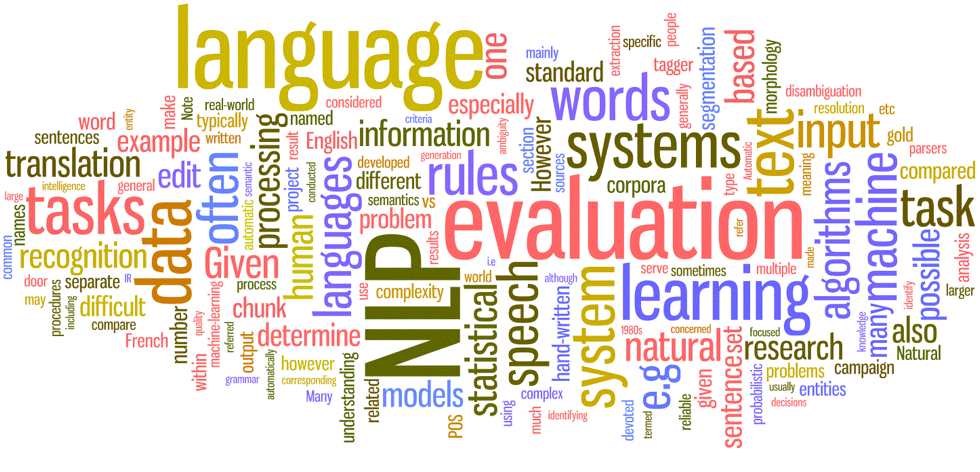
\includegraphics[width=7cm]{./figs/NLPTM_wordcloud.png}}

\end{frame}

%######################################################
%######################################################
\begin{frame}

	\frametitle{Natural Language Processing Applications}

\centerline{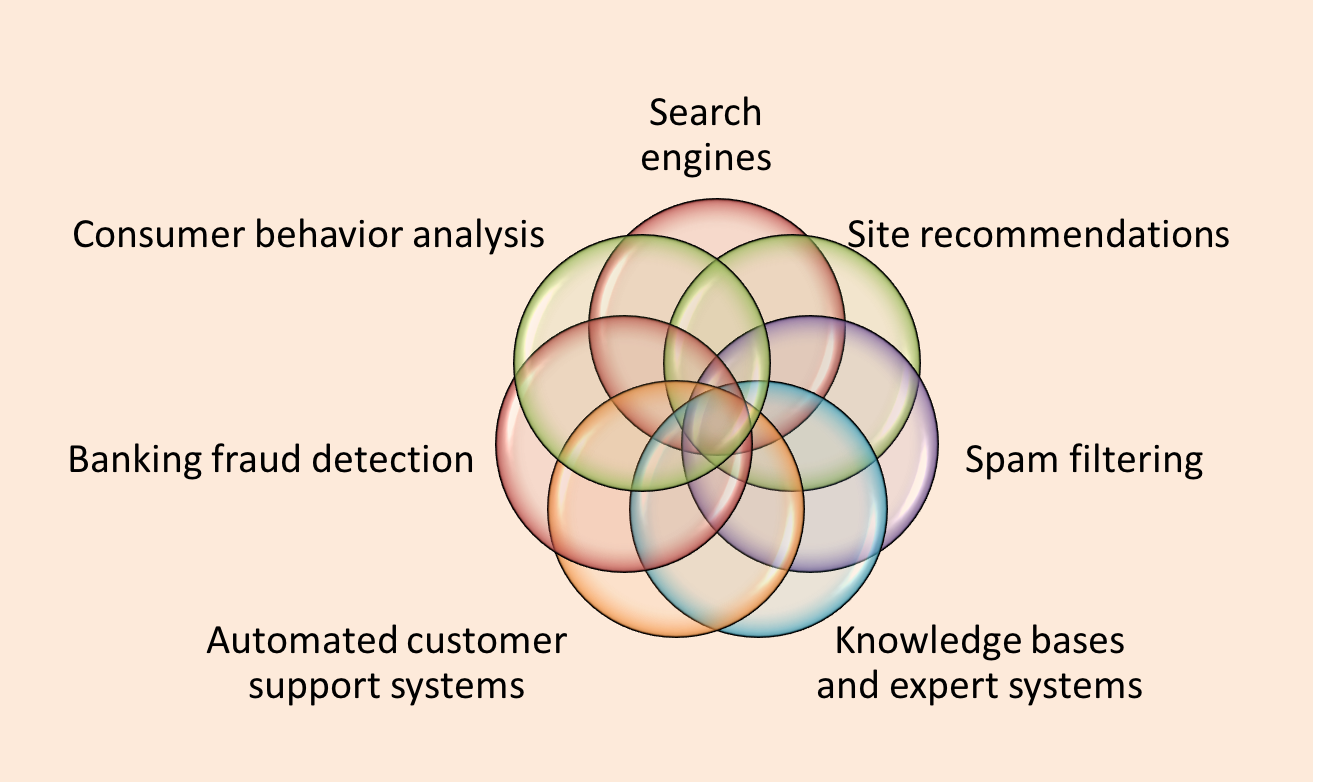
\includegraphics[width=9cm]{./figs/NLPTM_applications.png}}

\vspace{.3cm}
Here, we will pay attention to tools for the unsupervised {\bf semantic} organization of documental databases.

\end{frame}

%######################################################
%######################################################
\begin{frame}

	\frametitle{NLP challenges to machines}

	\large
	
	\begin{block}{Generic difficulties}
	\begin{itemize}
	
		\item Natural Language can be highly {\bf ambiguous}
		\item {\bf Disambiguation} of polysemic words
		\item {\bf Sentiment Analysis}
		\item {\bf Intention inference}: sarcasm, humor, etc
		\item Differentiate main from secondary topics
		\item Incorporate domain-expert knowledge into automatically inferred statistical models
	
	\end{itemize}
	\end{block}

	\begin{block}{Specific applications}
	\begin{itemize}
	
		\item Text summarization
		\item Machine dialog systems
	
	\end{itemize}
	\end{block}


\end{frame}


%######################################################
%######################################################
\subsection{Block overview}

%######################################################
%######################################################
\begin{frame}

	\frametitle{Module overview}

			We will study the topics for research funded by NSF during recent
			years, and infer thematic relations among institutions. We will


	\begin{columns}
	
	\begin{column}{.3\textwidth}
		\vspace{.2cm}
		\centerline{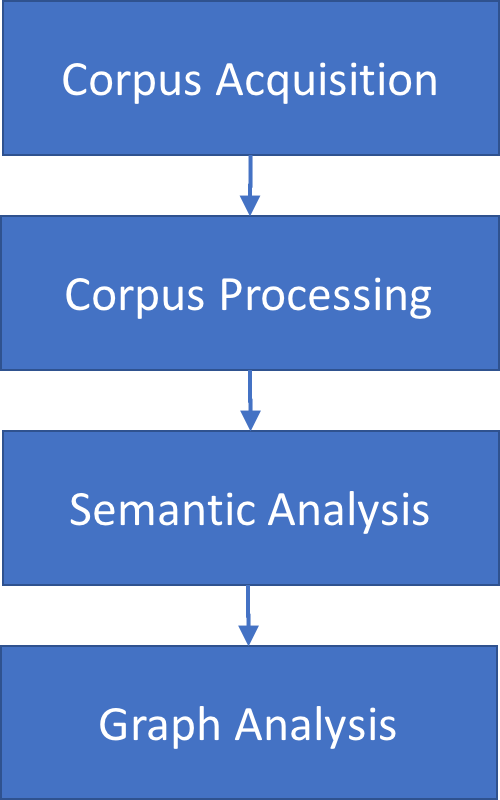
\includegraphics[width=.9\textwidth]{./figs/NLPTM_schema.png}}
	\end{column}
	
	\begin{column}{.6\textwidth}
		\begin{itemize}
			
			\item Discuss possibilities for corpus acquisition
			\item Present some of the most relevant text preprocessing techniques in the NLTK
			\item Present theoretical foundations and implementations of topic modeling algorithms
			\item Use the semantic representations to infer graphs among entities, and visualize them using Gephi	
			
		\end{itemize}
	\end{column}

	\end{columns}

\end{frame}



%######################################################
%######################################################
\begin{frame}

	\frametitle{Python libraries we will use}

	\begin{itemize}
		\item The Natural Language Processing Toolkit (NLTK)
		
		\url{http://www.nltk.org}
		
		Best for education and research, but not optimized for SW production
		
			\begin{itemize}
				\item Corpora	
				\item Entity recognition
				\item POS tagging
				\item Stemming and lemmatization
				\item Stopword lists
				\item + other text preprocessing and homogeneization tools
				 
			\end{itemize}
		
		\item Gensim
		
		\url{https://radimrehurek.com/gensim/}
		
		Library specialized on topic modeling and document similarity analysis

			\begin{itemize}
				\item Topic models: LDA, LSI	
				\item Word2vec and Doc2vec
				\item Pagerank
				 
			\end{itemize}


	\end{itemize}	


\end{frame}


%######################################################
%######################################################
\section{Corpus acquisition}

%######################################################
%######################################################
\begin{frame}

    \frametitle{Contents}

	\large

    \begin{enumerate}
  
    	\item {Overview and block objectives}
    	\item {\bf \color{blue}Corpus acquisition}
    	\item Corpus preprocessing, cleaning and homogeneization
    	\item Topic modeling with Latent Dirichlet Allocation
    	\item Graph tools
    
    \end{enumerate}

\end{frame}

%######################################################
%######################################################
\begin{frame}

    \frametitle{Text sources}

	There are many possibilities for acquiring interesting textual databases

	\begin{columns}
	
	\begin{column}{.5\textwidth}
		\begin{itemize}
			
			\item Web content (web pages, twitter, blogs, etc)
			\begin{itemize}
				\item Crawlers
				\item Available APIs (e.g., wikipedia, arXiv)
			\end{itemize}
			\item Local document collections
			\item Available corpus	
			
		\end{itemize}
	\end{column}
	
	\begin{column}{.5\textwidth}
		\vspace{.2cm}			\centerline{
\includegraphics[width=\textwidth]{./figs/NLPTM_wordcloud2.png}}
	\end{column}

	\end{columns}
	
Some applications examples
\begin{itemize}
\item Use job portals for modeling the job market in a country
\item Analyze innovation from patent descriptions
\item Categorize apps from their textual description in App stores
\item {\bf{Analyze public funding topics using projects abstracts}}
\end{itemize}

\end{frame}


%######################################################
%######################################################
\subsection{NSF dataset construction}


%######################################################
%######################################################
\begin{frame}

    \frametitle{National Science Foundation data}
    
	We will work with project description and metadata taken from the National Science Foundation website (\url{http://www.nsf.org}). The information is encoded in XML format, as shown in the example below:
	
	\vspace{.2cm}

	\centerline{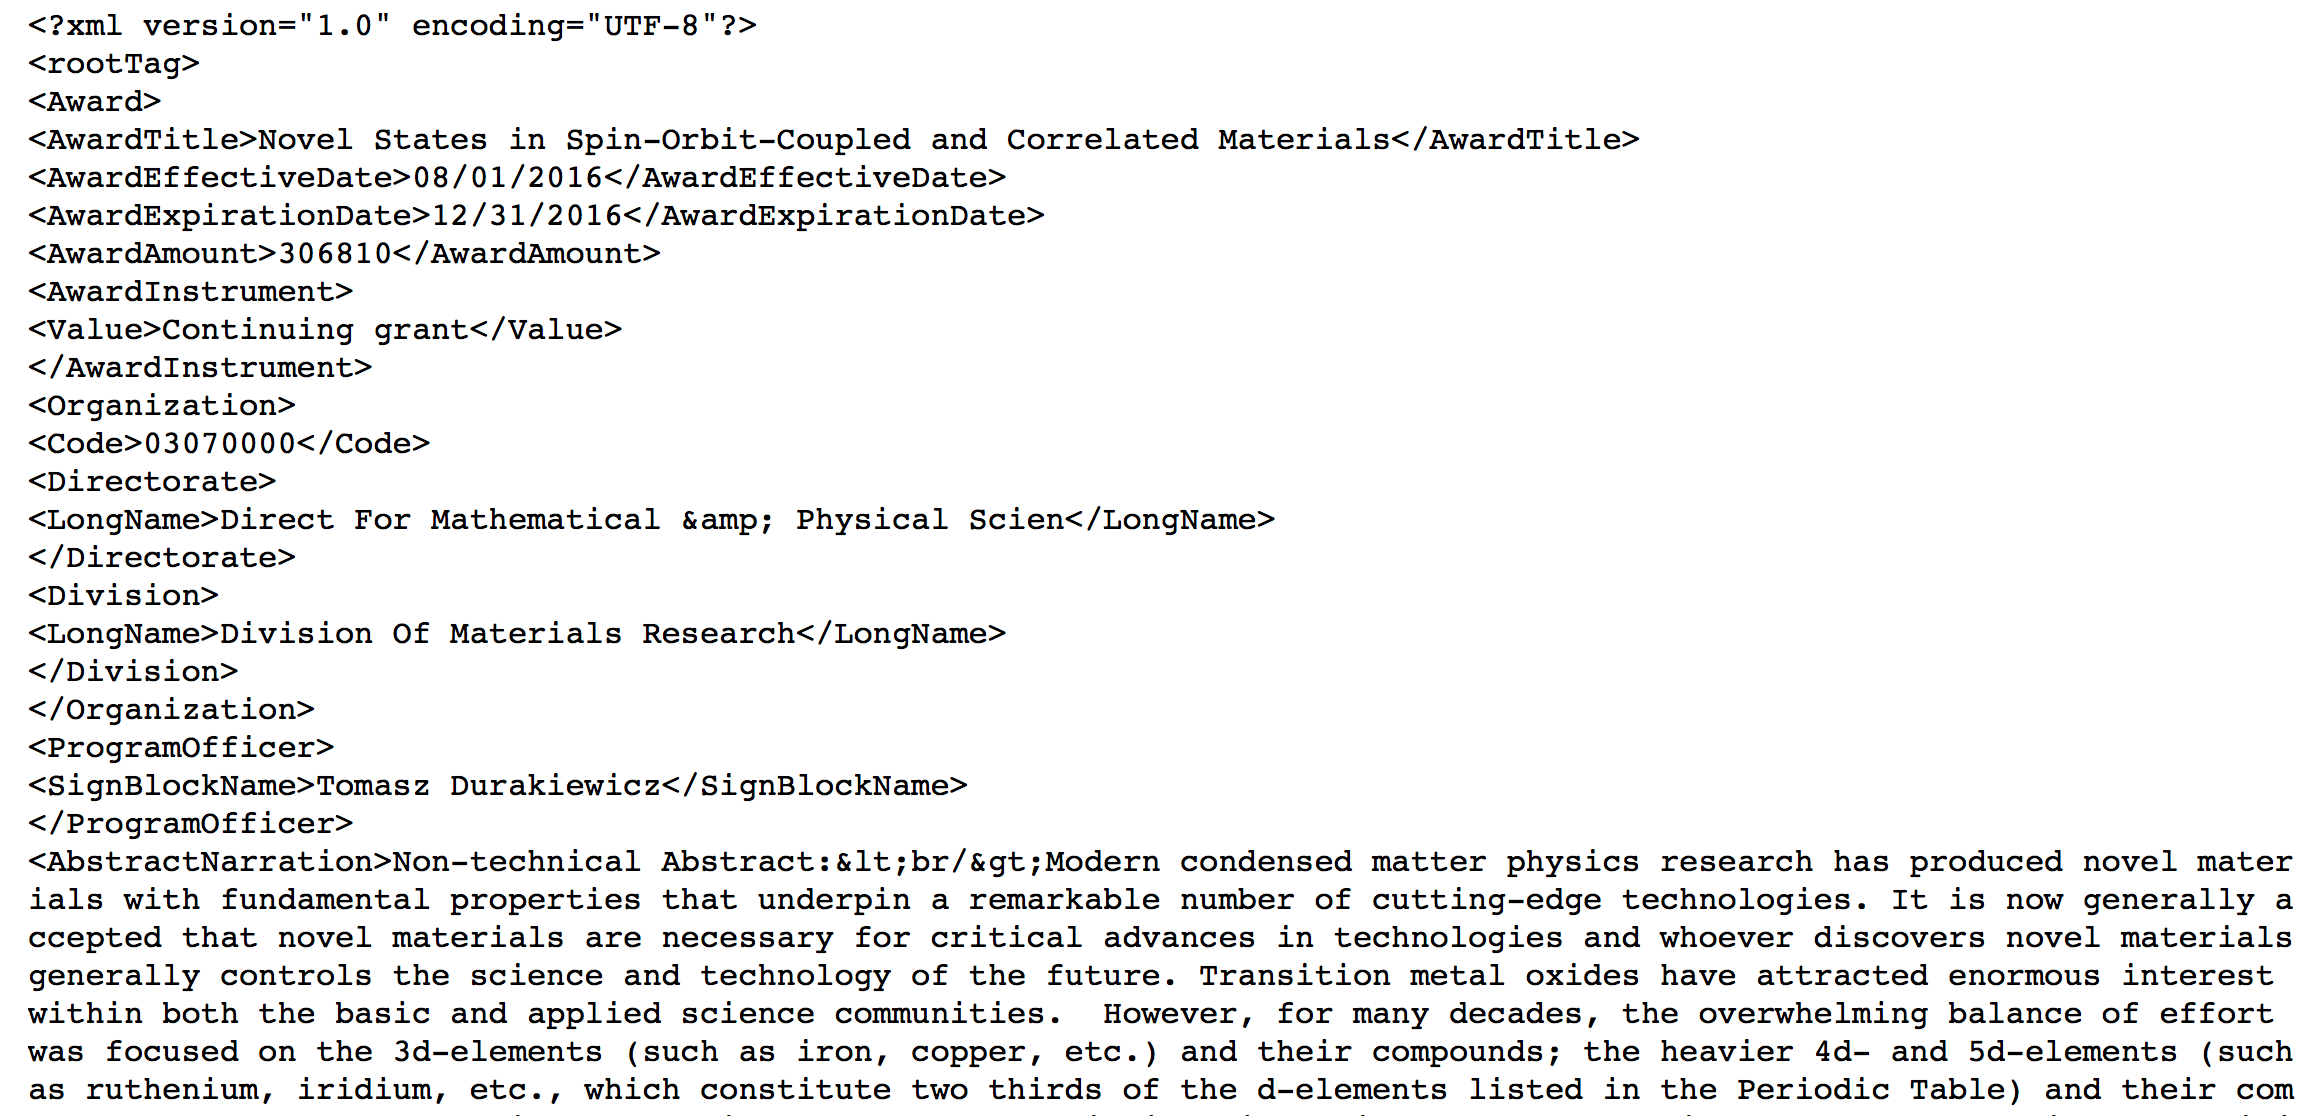
\includegraphics[width=\textwidth]{./figs/NLPTM_xml.png}}

\end{frame}

%######################################################
%######################################################
\begin{frame}

    \frametitle{NSF dataset construction}
    
	\begin{block}{Relevant files}
	
		\begin{itemize}
		
			\item Zip files under the `data' directory (contain compressed projects information and metadata)
			
			\item Python notebook `02901.ipynb'
			
		\end{itemize}
	
	\end{block}
	
	\begin{exampleblock}{Exercise}
		
			\begin{itemize}
			
				\item Go through subsections 1.1.1. and 1.1.2. that explain the basics of working with XML files in python
				
				\item Complete the exercise described in subsection 1.1.3. You have to implement a function that extracts the following information for each project:
				
				\begin{itemize}
					\item Text data (for semantic analysis): Title, Abstract
					\item Metadata: Budget, Starting Year, Institution
				\end{itemize}
				
				\item Go through the rest of Chapter 1 to see how the whole dataset is constructed and to understand its structure
				
			\end{itemize}
		
	\end{exampleblock}
	
\end{frame}


%######################################################
%######################################################
\section{Corpus preprocessing}

%######################################################
%######################################################
\begin{frame}

    \frametitle{Contents}

	\large

    \begin{enumerate}
  
    	\item Overview and block objectives
    	\item Corpus acquisition
    	\item {\bf \color{blue}Corpus preprocessing, cleaning and homogeneization}
    	\item Topic modeling with Latent Dirichlet Allocation
    	\item Graph tools
    
    \end{enumerate}

\end{frame}


%######################################################
%######################################################
\begin{frame}

    \frametitle{Document representation for Machine Learning}

    \begin{itemize}
  
    	\item ML algorithms process numbers, not words
    	\item We need to transform text into meaningful numbers
    	\item Bag-of-Words (BoW) representation: Count number of appearances of each word (in the vocabulary of all documents) in a given document
    	\item In order to have a useful representation, some preprocessing steps are normally required
    
    \end{itemize}
    
    \vspace{1cm}
    
    \centerline{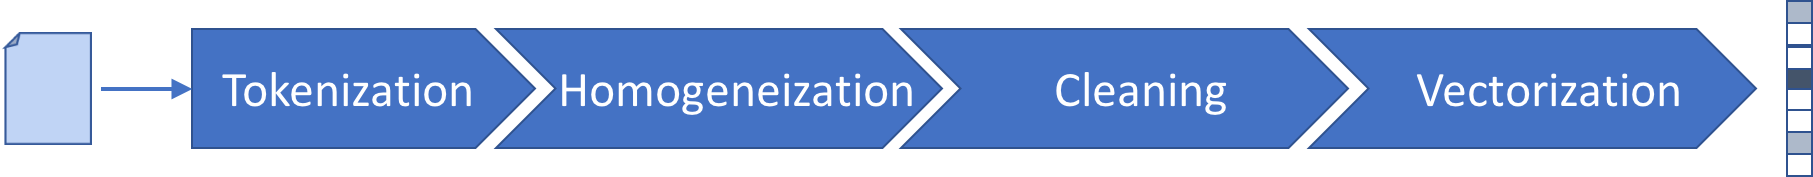
\includegraphics[width=\textwidth]{./figs/NLPTM_doc_preproc.png}}

\end{frame}


%######################################################
%######################################################
\subsection{Natural Language Processing Toolkit (NLTK)}

%######################################################
%######################################################
\begin{frame}

\frametitle{NLP with Python}

	\begin{columns}
	
	\begin{column}{.5\textwidth}
	
	NLTK: A package that provides:
	
		\begin{itemize}
			
			\item Basic classes for representing data relevant to natural language processing
			
			\item Functions for performing common NLP tasks (parsing, tokenization, etc)
			
			\item Corpuses (text collections, stopword lists, etc)
			
		\end{itemize}
	\end{column}
	
	\begin{column}{.5\textwidth}
		\vspace{.2cm}			\centerline{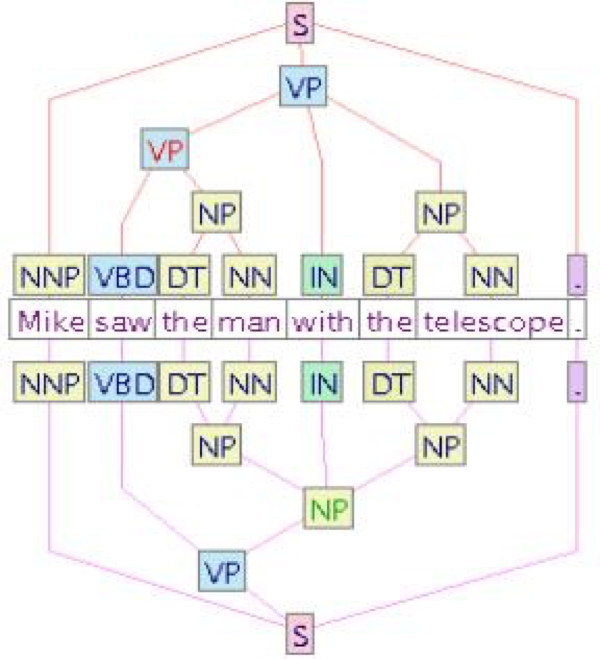
\includegraphics[width=\textwidth]{./figs/NLPTM_NLTKgeneral.png}}
	\end{column}

	\end{columns}
	

\end{frame}

%######################################################
%######################################################
\begin{frame}

\frametitle{NLTK modules}

	\begin{itemize}
			
		\item corpora: a package containing collections of example text 
		\item {\bf tokenize}: functions to split text strings into basic elements
		\item probability: for modeling frequency distributions and probabilistic systems 
		\item {\bf stem}:  package of functions to stem words of text 
		\item {\bf wordnet}: interface to the WordNet lexical resource 
		\item chunk: identify short non-nested phrases in text 
		\item etree: for hierarchical structure over text 
		\item {\bf tag}: tagging each word with part-of-speech, sense, etc. 
		\item parse: building trees over text - recursive descent, shift-reduce, probabilistic, etc. 
		\item cluster: clustering algorithms 
		\item draw: visualize NLP structures and processes 
		\item contrib: various pieces of software from outside contributors 

	\end{itemize}

\end{frame}


%######################################################
%######################################################
\subsection{Tokenization}

%######################################################
%######################################################
\begin{frame}

    \frametitle{Tokenization}

    \centerline{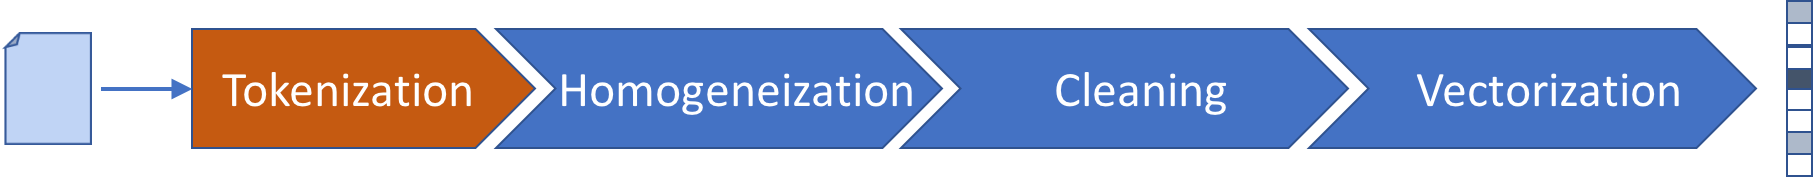
\includegraphics[width=\textwidth]{./figs/NLPTM_tokenization.png}}

    \begin{itemize}
  
    	\item The goal is to find the basic elements (tokens) of a given string. 
    	\item Python {\tt split()} function makes a list from a string using a given substring as a separator
    	\item NLTK tokenizers are better suited to this task, and more efficient since they use regular expressions.
    	
    \end{itemize}
    
    \begin{block}{Example}
    	\begin{itemize}
    		\footnotesize
    		\item[] $\gg$ {\tt sentence = 'Hello, world.'}
    		\item[] $\gg$ {\tt sentence.split()}
    		\item[] {\tt ['Hello,', 'world.']}
    		\item[] $\gg$ {\tt from nltk.tokenize import word\_tokenize}
    		\item[] $\gg$ {\tt tokens = word\_tokenize(sentence)}
    		\item[] $\gg$ {\tt tokens = [el for el in tokens if el.isalnum()]}
    		\item[] {\tt ['Hello', 'world']}
    	
    	\end{itemize}
    \end{block}
    
\end{frame}


%######################################################
%######################################################
\subsection{Homogenization}

%######################################################
%######################################################
\begin{frame}

    \frametitle{Homogenization}

    \centerline{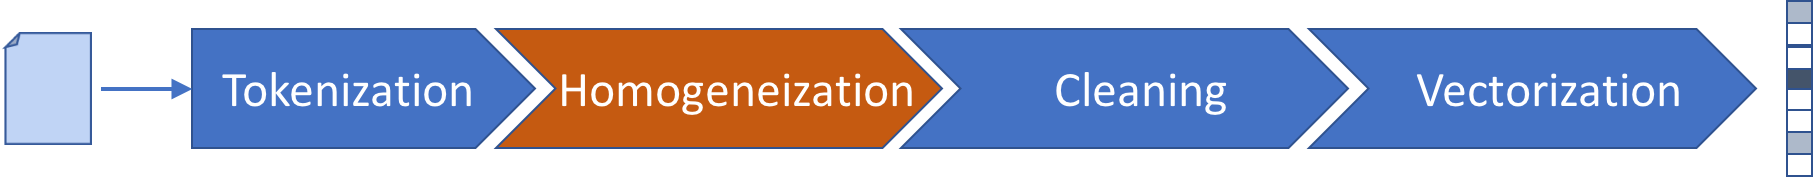
\includegraphics[width=\textwidth]{./figs/NLPTM_homogenization.png}}

    \begin{itemize}
    	\item The goal is collapse all equivalent words (i.e., semantically equivalent) in a unique representative
    		\begin{itemize}
    			\item Different forms of a word: \\ 
    			organize, organizes, organizing, ... $\rightarrow$ organize 
    			\item Derivationally related words with similar meanings: \\ democracy, democratic, democratization, ... $\rightarrow$ democracy
    		\end{itemize}
    		
    	\item Stemming vs lemmatization
    		\begin{itemize}
    			\item {\bf Stemming} chops of the ends of words using a list of suffixes
    			\item {\bf Lemmatization} usually refers to doing things properly with a vocabulary and morphological analysis of words, aiming to return the base or dictionary form (lemma) of a word. 
				\item A practical difference is that lemmatizers output complete words.

    		\end{itemize}
    		
    	\item If using case sensitive implementations, we need to lowercase the tokens as a preliminary step
    	
    \end{itemize}
    
\end{frame}


%######################################################
%######################################################
\begin{frame}

    \frametitle{Stemming}

    	\begin{itemize}
    		\item[] $\gg$ {\tt import nltk.stem}
    		\item[] $\gg$ {\tt s = nltk.stem.SnowballStemmer('english')}
    		\item[] $\gg$ {\tt s.stem('image')} $\rightarrow$ {\tt 'imag'}
    		\item[] $\gg$ {\tt s.stem('images')} $\rightarrow$ {\tt 'imag'}
    		\item[] $\gg$ {\tt s.stem('organize')} $\rightarrow$ {\tt 'organ'}
    		\item[] $\gg$ {\tt s.stem('organizing')} $\rightarrow$ {\tt 'organ'}
			\item[] $\gg$ {\tt s.stem('organ')} $\rightarrow$ {\tt 'organ'}
    	\end{itemize}

\end{frame}


%######################################################
%######################################################
\begin{frame}

    \frametitle{Lemmatization}
    
    	\begin{block}{}
    	\begin{itemize}
    	\item NLTK recurs to WordNet, a lexical database for the English language. Wordnet groups English words into sets of synonyms called synsets.
    	\item With contextual information (the grammatical role of the word) {\tt lemmatize()} can filter grammatical differences
    	\end{itemize}
    	\end{block}
    	
    	\begin{itemize}
    		\footnotesize
    		\item[] $\gg$ {\tt from nltk.stem import WordNetLemmatizer}
    		\item[] $\gg$ {\tt wnl = WordNetLemmatizer()}
    		\item[] $\gg$ {\tt wnl.lemmatize('image')} $\rightarrow$ {\tt 'image'}
    		\item[] $\gg$ {\tt wnl.lemmatize('images')} $\rightarrow$ {\tt 'image'}
    		\item[] $\gg$ {\tt wnl.lemmatize('organize')} $\rightarrow$ {\tt 'organize'}
    		\item[] $\gg$ {\tt wnl.lemmatize('organizing')} $\rightarrow$ {\tt 'organizing'}
    		\item[] $\gg$ {\tt wnl.lemmatize('organizing', pos='v')} $\rightarrow$ {\tt 'organize'}
    		\item[] $\gg$ {\tt wnl.lemmatize('organ')} $\rightarrow$ {\tt 'organ'}
       	\end{itemize}
    
\end{frame}


%######################################################
%######################################################
\begin{frame}

    \frametitle{Other homogeneization tasks}
    
    	\begin{block}{Part of Speech Tagging}
    	\begin{itemize}
    	\item Part-of-speech (POS) tagging is the process of assigning a word to its grammatical category (noun, verb, adverb,…), in order to understand its role within the sentence.
    	\item POS tagging is provides the contextual information to {\tt lemmatize()} to filter grammatical differences.

    	\end{itemize}
    	\end{block}
    	
    	\begin{itemize}
    		\footnotesize
    		\item[] $\gg$ {\tt from nltk import pos\_tag}
    		\item[] $\gg$ {\tt tokens = word\_tokenize('This is a simple sentence') }
    		\item[] $\gg$ {\tt pos\_tag(tokens)}
    		\item[] {\tt [('This', 'DT'), ('is', 'VBZ'), ('a', 'DT'), ('simple', 'JJ'), ('sentence', 'NN')]}
       	\end{itemize}
    
    	\begin{block}{N-gram detection}
        	\begin{itemize}
        	\item Identification of groups of words that occasionally appear together, and have an inherent semantic value
        	\item E.g.: Machine learning, big data, etc
        	\end{itemize}
        \end{block}
    
\end{frame}


%######################################################
%######################################################
\subsection{Cleaning}

%######################################################
%######################################################
\begin{frame}

    \frametitle{Cleaning}

    \centerline{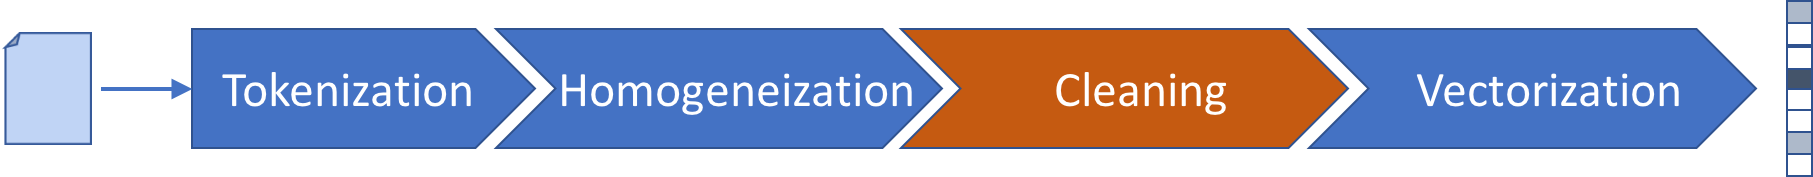
\includegraphics[width=\textwidth]{./figs/NLPTM_cleaning.png}}

    The goal is to remove irrelevant words
    		\begin{itemize}
    			\item Stopwords: Words that appear very often in all sorts of different contexts. They are removed by using stopwords lists
    			\item Very rare terms: We may also want to remove words that appear in a very reduced number of documents in the collection
    			\item Very common terms: We may also want to remove words that, in spite of not being stopwords, are very common for a particular dataset, or simply do not have significant semantic value for the application at hand
    		\end{itemize}
    			
    
\end{frame}


%######################################################
%######################################################
\subsection{Vectorization}

%######################################################
%######################################################
\begin{frame}

    \frametitle{Vectorization: Bag-of-words representation}

    \centerline{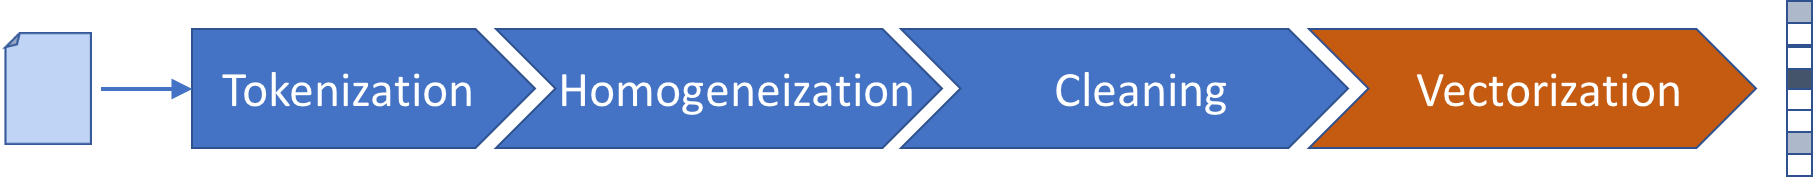
\includegraphics[width=\textwidth]{./figs/NLPTM_vectorization.png}}

    The goal is to convert the sequence of homogenized and cleaned tokens into a numeric vector
    \begin{itemize}
    	\item Bag-of-words representation: counts how many appearances of each word occur in each document
    	\item Each position in the vector is associated to a unique word in the vocabulary, so vectors are typically very sparse
    \end{itemize}
    
    \vspace{.2cm}
    \centerline{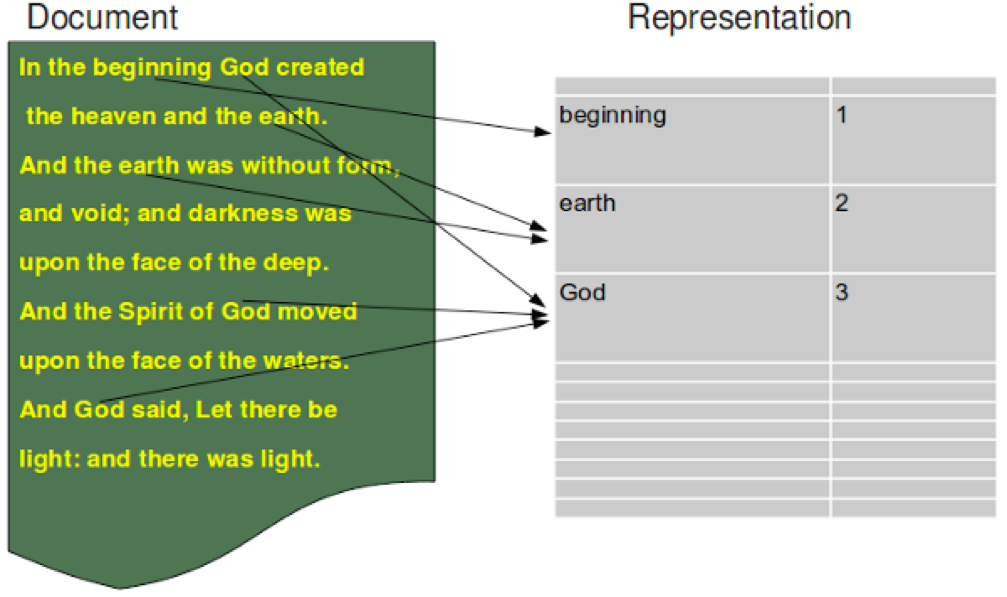
\includegraphics[width=.5\textwidth]{./figs/NLPTM_BoW.png}}
    			    
\end{frame}


%######################################################
%######################################################
\begin{frame}

    \frametitle{Term frequency - Inverse document frequency (TF-IDF)}

    We want a high value for a given term in a given doc if that term occurs often in that particular doc and very rarely anywhere else

	\begin{itemize}
	
	\item ${\rm TF}(w,d) = \frac{{\rm BoW}(w,d)}{\# {\text{ words in } d}}$
	\item ${\rm IDF}(w) = \log \frac{\# {\text{ docs}}}{\# {\text{ docs with term } w}}$
	\item ${\rm TF-IDF}(w,d) = {\rm TF}(w,d) \times {\rm IDF}(w)$
		
	\end{itemize}
	
	The IDF term emphasizes the words that appear in a reduced number of documents.
    			    
\end{frame}


%######################################################
%######################################################
\subsection{Exercises}

%######################################################
%######################################################
\begin{frame}

    \frametitle{Exercises}

    \begin{exampleblock}{Exercise}
	
	\begin{itemize}
		\item Preprocess the text data in the NSF dataset, completing all the steps that have been reviewed in the presentation
		\item Follow Chapter 2 of the provided `DTU02901.ipynb` notebook. As a result, the following variables will be available:
		
		\begin{itemize}
			\item {\tt D}: A gensim dictionary. Term strings can be accessed using the numeric identifiers. For instance, {\tt D[0]} contains the string corresponding to the first position in the BoW representation.
			\item {\tt corpus\_bow}: BoW corpus. A list containing an entry per project in the dataset, and consisting of the (sparse) BoW representation for the abstract of that project.
			\item {\tt NSF\_data}: A list containing an entry per project in the dataset, and consisting of metadata for the projects in the dataset
		\end{itemize}
		
	\end{itemize}
	\end{exampleblock}
				    
\end{frame}


%######################################################
%######################################################
\section{Topic Modeling with LDA}

%######################################################
%######################################################
\begin{frame}

    \frametitle{Contents}

	\large

    \begin{enumerate}
  
    	\item Overview and block objectives
    	\item Corpus acquisition
    	\item Corpus preprocessing, cleaning and homogeneization
    	\item {\bf \color{blue}Topic modeling with Latent Dirichlet Allocation}
    	\item Graph tools
    
    \end{enumerate}

\end{frame}


%######################################################
%######################################################
\subsection{Topic Models}

%######################################################
%######################################################
\begin{frame}

    \frametitle{Topic models}

	\large

    \begin{itemize}
  
    	\item Topic Models attempt to uncover the underlying semantic structure of a document corpus by identifying recurring patterns of terms (topics).
    	\item Topic models are models for bags-of-words:
    	\begin{itemize}
			\item do not parse sentences
			\item do not care about word order, and
			\item do not ``understand'' grammar or syntax
		\end{itemize}
		\item Topic models are useful on their own to build visualizations and explore data. They are also very useful as an intermediate step in many other tasks.

    
    \end{itemize}

\end{frame}


%######################################################
%######################################################
\begin{frame}

    \frametitle{Topic modeling tools}

	\begin{itemize}
  
    	\item {\bf Gensim} is an NLP toolbox Developed by Radim Rehurek, and specialized in topic modeling and semantic analysis of texts. It includes:
    	\begin{itemize}
			\item Tools for BoW codification of documents
			\item Tools for TF-IDF representation of documents
			\item Latent Semantic Indexing (LSA/LSI)
			\item {\bf Latent Dirichlet Allocation (LDA)}
			\item Dynamic topic modeling (incomplete)
			\item Word2Vec tools for mapping words in a vector semantic space
		\end{itemize}
		\item In the block we will rely on David Blei's LDA algorithm that rely on the BoW representations. Other available Python implementations are:
		\begin{itemize}
			\item LDA toolbox
			\item Scikit learn implementation
			\item GraphLab (based on collapsed Gibbs sampling)
		\end{itemize} 
		\item MALLET contains a well-known Java implementation of LDA
    
    \end{itemize}

\end{frame}

%######################################################
%######################################################
\begin{frame}

    \frametitle{Topic model visualizers}

	Given the extended use of topic models, some researchers have also publish tools for visualizing the results of topic models.

    \begin{itemize}
  
    	\item dfr-browser: \url{https://github.com/agoldst/dfr-browser} \\
    	Demo: \url{https://agoldst.github.io/dfr-browser/demo/}
    	
    	\item pyLDAvis: \url{https://github.com/bmabey/pyLDAvis} \\
    	
    	\item Topic model visualization Engine (TMVE): \url{https://github.com/ajbc/tmve-original} \\
    	Demo: \url{http://www.princeton.edu/~achaney/tmve/wiki100k/browse/topic-presence.html} 
    
    \end{itemize}

\end{frame}


%######################################################
%######################################################
\subsection{LDA}

%######################################################
%######################################################
\begin{frame}

    \frametitle{Latent Dirichlet Allocation}

	\centerline{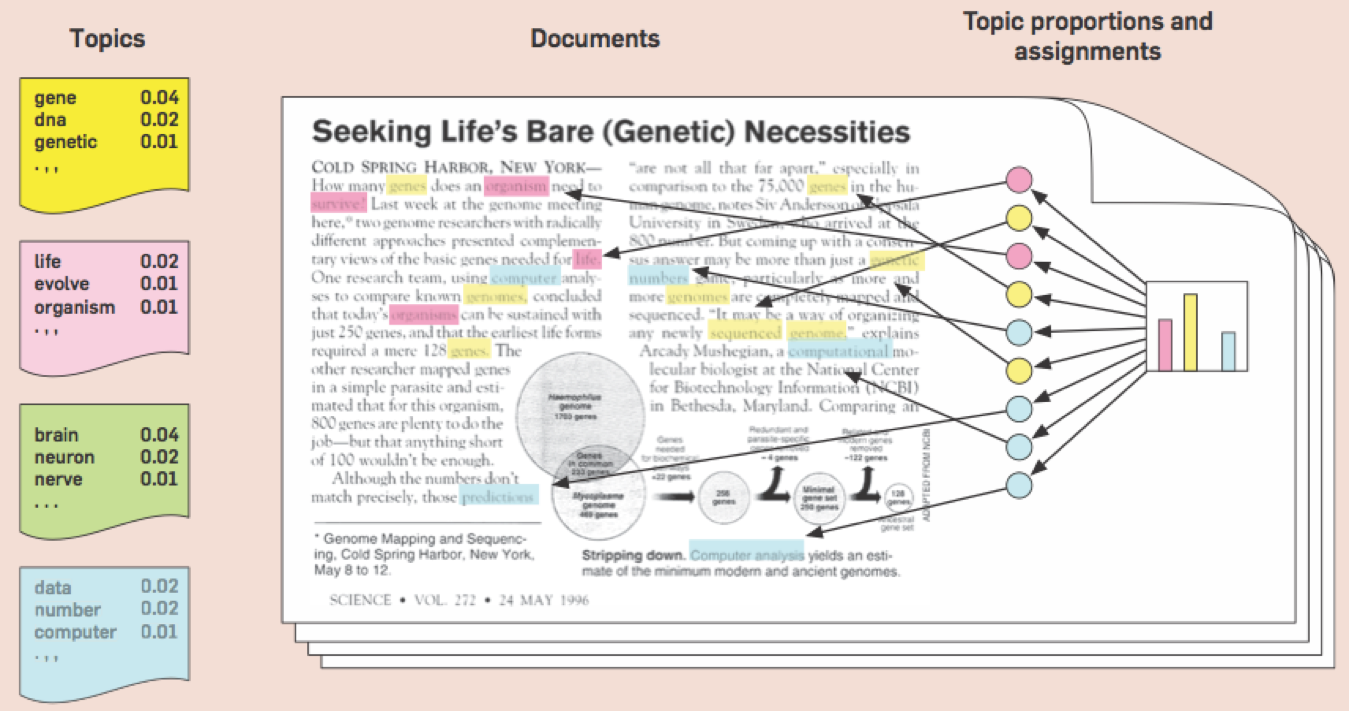
\includegraphics[width=\textwidth]{./figs/NLPTM_LDA.png}}
(Image taken from \url{http://www.cs.columbia.edu/~blei/papers/Blei2012.pdf})

\end{frame}

%######################################################
%######################################################
\begin{frame}

    \frametitle{Understanding LDA}

	LDA is a generative probabilistic model: 
	\begin{itemize}
	\item It assumes that documents have been generated according to some probability model with some unknown parameters an certain hidden variables
	
	\item The corpus data is used to infer the topic structure (hidden variables) from the words of documents (observed variables)
	\end{itemize}


	\centerline{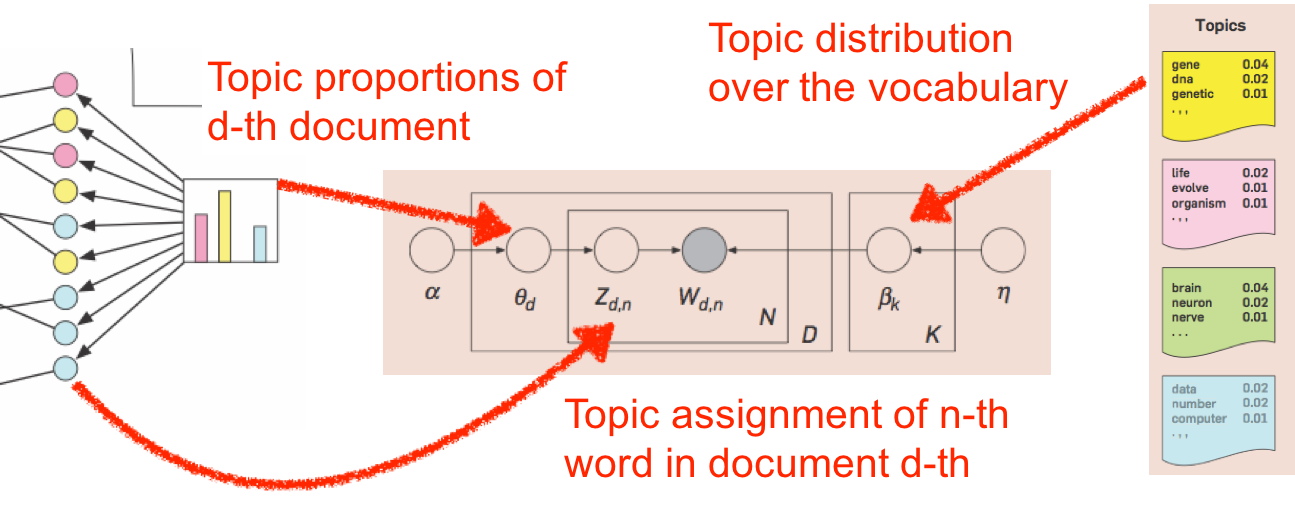
\includegraphics[width=.7\textwidth]{./figs/NLPTM_LDA2.png}}

\end{frame}


%######################################################
%######################################################
\begin{frame}

    \frametitle{LDA generative model}

	\centerline{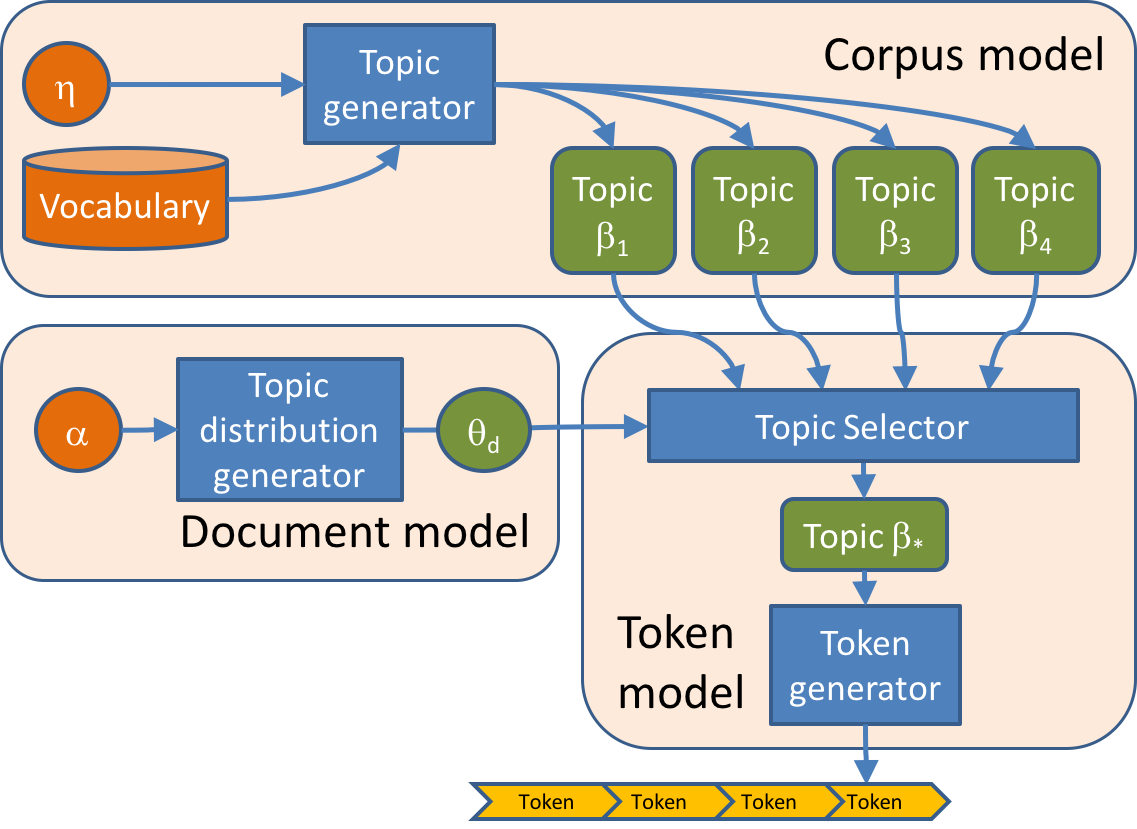
\includegraphics[width=.9\textwidth]{./figs/NLPTM_LDA3.png}}

\end{frame}

%######################################################
%######################################################
\begin{frame}

    \frametitle{LDA generative model (II)}

	\begin{itemize}
	\item Topic generator:
	\begin{itemize}
	\item Generates tokens distributions by means of a Dirichlet distribution with concentration parameter $\eta$.
	\item Each topic is therefore characterized by a vector $\boldsymbol{\beta}_t$ that indicates the term distribution for the given topic
	\item Large $\eta$ implies that topic distributions will be concentrated in a few distinct tokens (only a few non-zero components in each $\boldsymbol{\beta}_t$).
	\end{itemize}
	\item Document generator:
	\begin{itemize}
	\item For each document, generate its topic distribution by sampling a Dirichlet distribution with concentration parameter $\alpha$.
	\item Large $\alpha$ implies that for most documents only a few topics will be relevant.
	\item For each word in the document:
	\begin{itemize}
		\item Select a topic according to the topic distribution for the document
		\item Select a word from the word distribution for the selected topic
	\end{itemize}

	\end{itemize}

	\end{itemize}

\end{frame}

%######################################################
%######################################################
\begin{frame}

    \frametitle{LDA generative model (III)}

	\small
	\begin{itemize}
	\item The generative process for LDA corresponds to the following joint distribution of the hidden and observed variables
	\footnotesize
	$$p({\boldsymbol{\beta}}_{1:K}, {\boldsymbol{\theta}}_{1:D}, {\bf z}_{1:D}, w_{1:D}) = \prod_{i=1}^K p({\boldsymbol{\beta}}_i) \prod_{d=1}^D p({\boldsymbol{\theta}}_d) \left( \prod_{n=1}^{N_d} p({z}_{d,n}|{\boldsymbol{\theta}}_d) p({w}_{d,n} | {z}_{d,n}, {\boldsymbol{\beta}}_{1:K}) \right)$$
	

	\small
	\item Goal: computing the conditional distribution of the topic structure given the observed documents
	\footnotesize
	$$p({\boldsymbol{\beta}}_{1:K}, {\boldsymbol{\theta}}_{1:D}, {\bf z}_{1:D} | w_{1:D}) = \frac{p({\boldsymbol{\beta}}_{1:K}, {\boldsymbol{\theta}}_{1:D}, {\bf z}_{1:D}, w_{1:D})}{p(w_{1:D})}$$
	\small
	\item The denominator is the probability of seeing the observed corpus under any topic model. It can be computed by summing the joint distribution over every possible hidden topic structure, so its computation is not feasible.
	\item LDA implementations are based on:
	\begin{itemize}
	\item Variational Bayes implementations
	\item Sampling-based algorithms (typically, collapsed Gibbs-sampling with the goal of estimating word-assignments, ${\bf z}_{1:D}$)
	\end{itemize}
	
	\end{itemize}

\end{frame}

%######################################################
%######################################################
\subsection{Topic visualization}

%######################################################
%######################################################
\begin{frame}

    \frametitle{Topic visualization using pyLDAvis}

	\centerline{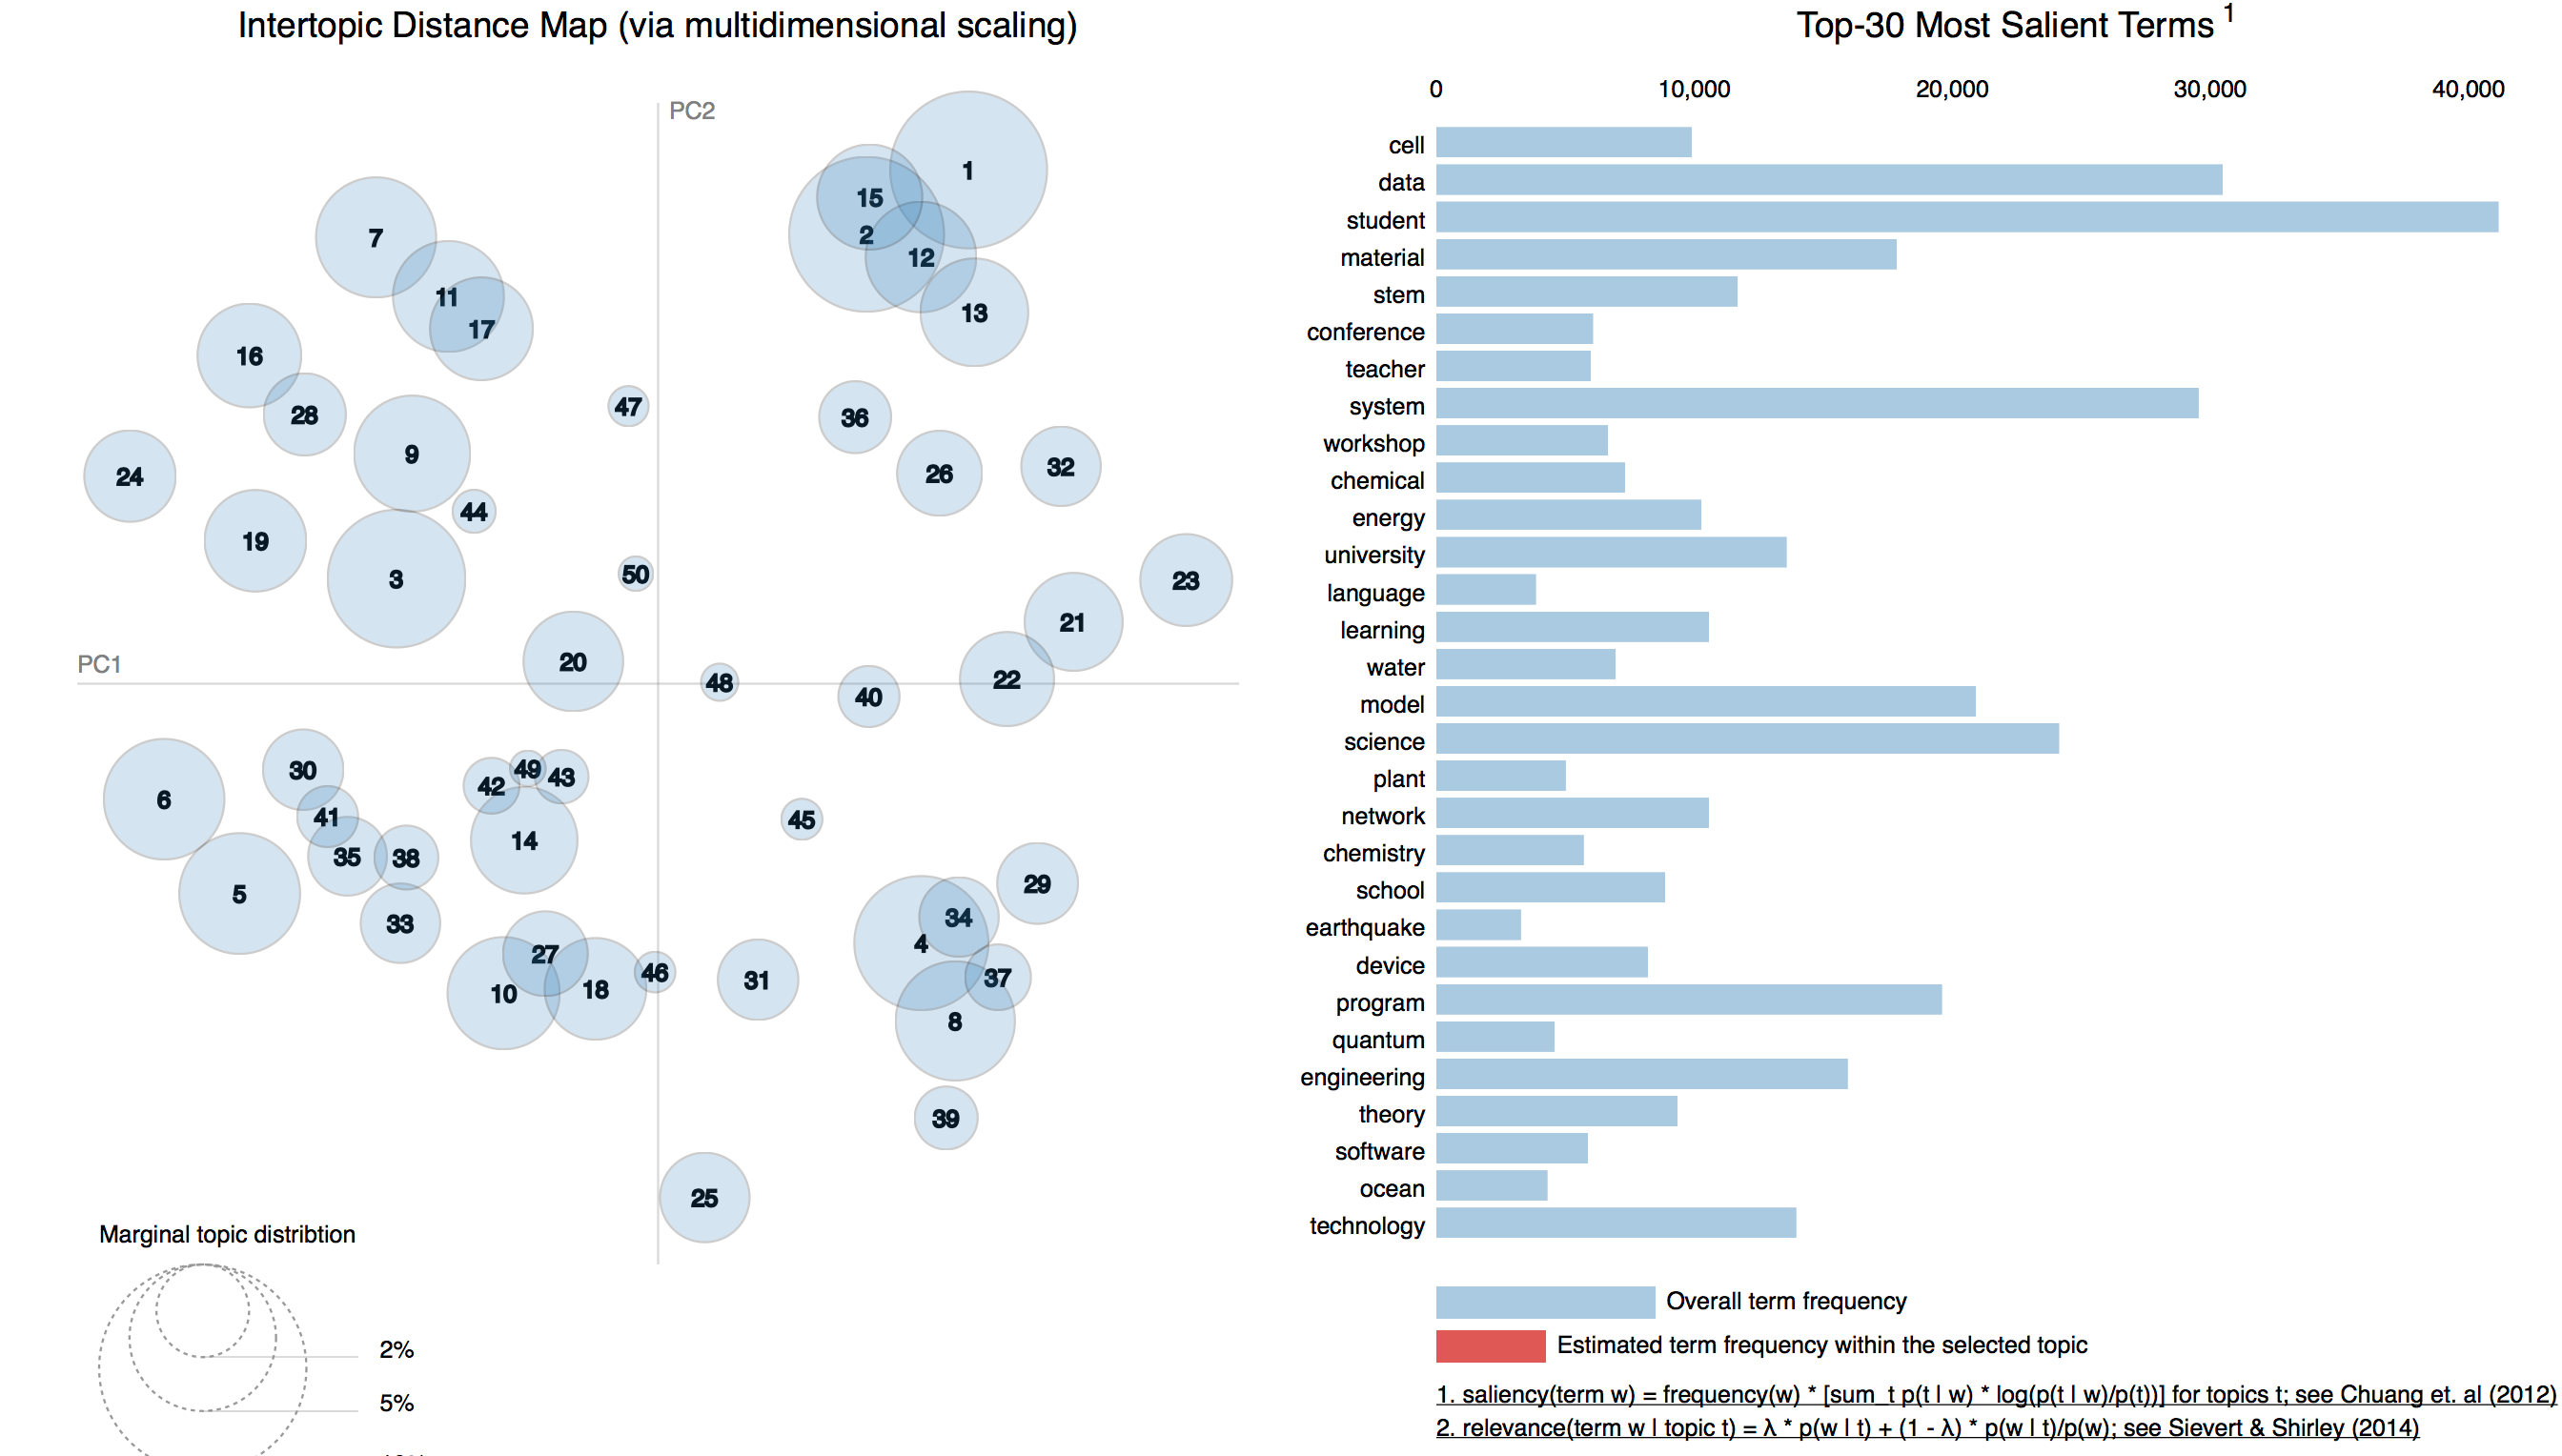
\includegraphics[width=\textwidth]{./figs/NLPTM_pyLDAvis.png}}
	
\end{frame}


%######################################################
%######################################################
\subsection{Open issues}

%######################################################
%######################################################
\begin{frame}

    \frametitle{Some open issues in topic modeling}

	\begin{itemize}
		\item Joint use of Topic Models and Word2Vec
		\begin{itemize}
			\item Word2Vec provides a semantically inspired vector representation of words
			\item Using this representation space, models can be aware of statistical dependencies among words
			\item Word2Vec relies on Deep Learning. The representation is given by the hidden layer of a network trained to predict words context.
		\end{itemize}
		\item Matching the topics of models trained with heterogeneous vocabularies
		\item Interactive topic models incorporating domain-expert knowledge
	\end{itemize}
	
\end{frame}

%######################################################
%######################################################
\subsection{Exercises}

%######################################################
%######################################################
\begin{frame}

    \frametitle{Exercises}

	\begin{exampleblock}{}
		\begin{itemize}
		\item Complete notebook subsections 3.1. and 3.2., and study how Topic Models can be trained and visualized using Gensim and pyLDAvis modules.
		\item Complete notebook subsection 3.4. to know about some useful Gensim functions to work with the topic model
		\item Complete the exercises in Subsection 3.4.
		\begin{itemize}
			\item Build a function that returns the most relevant projects for a given topic
			\item Build a function that computes the semantic distance between any two selected projects.
			\item Compute the distance between institutions as the median of all distances among all projects of both institutions
		\end{itemize}
	\end{itemize}
	\end{exampleblock}
	
\end{frame}


%######################################################
%######################################################
\section{Graph Analysis}

%######################################################
%######################################################
\begin{frame}

    \frametitle{Contents}

	\large

    \begin{enumerate}
  
    	\item Overview and block objectives
    	\item Corpus acquisition
    	\item Corpus preprocessing, cleaning and homogeneization
    	\item Topic modeling with Latent Dirichlet Allocation
    	\item {\bf \color{blue}Graph tools}
    
    \end{enumerate}

\end{frame}


%######################################################
%######################################################
\begin{frame}

    \frametitle{Graph Analysis}

	\begin{itemize}
  
    	\item We are in a position to build graphs to visualize and explore relationships among projects and institutions
    	
    	\item Project graphs:

	    	\begin{itemize}
	    		\item Each project is a network node, and the metadata is already available in the constructed dataset.
	    		\item The weight of the link between any two nodes can be computed from their JS divergence as
	    		$$exp(-\gamma \cdot \text{divergence})$$
	    		\item It is convenient to impose a threshold value to obtain a sparser graph.
    		\end{itemize}
    
    	\item Institution graphs:
    	
    		 \begin{itemize}
    		    		\item Each institution is a network node, and the metadata is already available in the constructed dataset.
    		    		\item The weight of the link between any two nodes can be computed as the mean (or median value) of 
    		    		$$exp(-\gamma \cdot \text{divergence})$$
    		    		for any pair of projects from the two institutions
    	    \end{itemize}
    \end{itemize}

\end{frame}


%######################################################
%######################################################
\begin{frame}

    \frametitle{Assignment}

	\begin{itemize}
  
    	\item Generate a graph of projects and/or institutions using the topic model you build during the session
    	\item If necessary, you can sample the nodes
    	\item Visualize the graph using Matlab tools of the Gephi software, and run any community detection algorithm to group projects or institutions that are semantically similar
    	
    \end{itemize}

\end{frame}





\end{document} 